\subsection{二値化閾値の自動決定 --- 固定閾値と大津の方法の比較}

課題 8 の {\tt binarize\_frame} は、グレースケール値が 128 以上の画素を白、
それ未満を黒とする固定閾値方式で二値化している。閾値 128 は 8 bit 階調の
中央という以外に入力への根拠を持たないため、この設計選択の妥当性を、
ヒストグラムから閾値を自動決定する大津の方法(判別分析法)と比較して
定量的に評価した(実験ソースは付録の {\tt exp06\_otsu.py})。対象は
課題 8 で二値化動画の入力とした Cat - 66004.mp4(1280$\times$720、
294 フレーム、29.97 fps)である。比較する方式は次の 3 つである。

\begin{enumerate}
\item 固定 128: 課題 8 の採用手法。全フレームで閾値 128 を用いる。
\item フレーム毎 Otsu: 各フレームのヒストグラムから大津の方法で
      閾値を決め直す。
\item 動画一括 Otsu: 全 294 フレームのヒストグラムを合算した 1 つの
      ヒストグラムに大津の方法を 1 回だけ適用し、得た閾値を全フレームで
      共通に用いる。
\end{enumerate}

\subsubsection{大津の方法の原理}

大津の方法は 1979 年に大津展之が提案した閾値決定法で、画像の
ヒストグラムのみを入力とする大局的閾値法である。2025 年の文書画像
二値化のレビュー \cite{b6-binreview} でも、最も広く使われる閾値法の
一つとして挙げられている。

グレースケール値 $i\ (i = 0, \ldots, 255)$ の正規化ヒストグラム
(相対度数)を $p_i$ とし、閾値 $t$ で画素を
クラス $C_0 = \{0, \ldots, t\}$ とクラス $C_1 = \{t+1, \ldots, 255\}$ に
分けると、各クラスの生起確率は

\begin{equation}\label{eq:b6-omega}
\omega_0(t) = \sum_{i=0}^{t} p_i, \qquad
\omega_1(t) = 1 - \omega_0(t)
\end{equation}

であり、累積 1 次モーメント $\mu(t) = \sum_{i=0}^{t} i\,p_i$ と
全体平均 $\mu_T = \mu(255)$ を用いると、各クラスの平均は

\begin{equation}\label{eq:b6-mu}
\mu_0(t) = \frac{\mu(t)}{\omega_0(t)}, \qquad
\mu_1(t) = \frac{\mu_T - \mu(t)}{\omega_1(t)}
\end{equation}

と書ける。大津の方法は、クラス間分散

\begin{equation}\label{eq:b6-sigmab}
\sigma_B^2(t)
= \omega_0(t)\,\omega_1(t)\,\bigl(\mu_0(t) - \mu_1(t)\bigr)^2
= \frac{\bigl(\mu_T\,\omega_0(t) - \mu(t)\bigr)^2}
       {\omega_0(t)\bigl(1 - \omega_0(t)\bigr)}
\end{equation}

を最大にする閾値

\begin{equation}\label{eq:b6-argmax}
t^{*} = \mathop{\rm arg\,max}_{0 \le t < 255} \sigma_B^2(t)
\end{equation}

を選ぶ。画像全体の分散 $\sigma_T^2$ は $t$ に依存せず、クラス内分散
$\sigma_W^2(t)$ との間に $\sigma_T^2 = \sigma_W^2(t) + \sigma_B^2(t)$ が
成り立つから、クラス間分散の最大化はクラス内分散の最小化、すなわち
「2 クラスそれぞれが最も均質になる分割」の選択と等価である。
二値化は $\mathit{gray} > t^{*}$ を白とする(OpenCV と同じ規約。
課題 8 の固定閾値 $\mathit{gray} \ge 128$ はこの規約で $t = 127$ に
相当する)。

\subsubsection{自作実装と OpenCV 実装の一致検証}

式 \ref{eq:b6-omega}〜\ref{eq:b6-argmax} を numpy で実装した
(関数 {\tt otsu\_threshold})。ヒストグラムを {\tt np.bincount} で
求めたのち、式 \ref{eq:b6-omega} と $\mu(t)$ を {\tt np.cumsum} で
一括計算すれば、256 通りすべての $t$ に対する式 \ref{eq:b6-sigmab} が
配列演算 1 回で得られる。画素数 $N$、階調数 $L = 256$ に対して
計算量は $O(N + L)$ であり、$t$ ごとにヒストグラムを走査する素朴な
実装の $O(N + L^2)$ より効率がよい。最大値が複数の $t$ で並ぶ場合は
{\tt np.argmax} が最初の位置を返すため最小の $t$ が選ばれ、OpenCV の
実装と同じ規約になる。

検証として、全 294 フレームで自作実装の閾値と
{\tt cv2.threshold} の {\tt THRESH\_OTSU} が返す閾値を比較した結果、
294 フレームすべてで一致し、差の最大値は 0 であった
({\tt cv2} は本課題の制約により提出プログラムでは使用せず、
この検証のための参考としてのみ用いた)。したがって以降の分析は
自作実装の閾値に基づく。計算時間は自作実装が 1 フレームあたり
40.7 ms、{\tt cv2} は二値化画像の生成まで含めて 6.5 ms(参考値)で
あった。自作実装の時間の大半は約 92 万画素のヒストグラム集計であり、
256 要素の累積和と最大値探索の時間は無視できる。フレーム間隔
$1/29.97 \approx 33.4$ ms と比べると、自作実装をそのまま毎フレーム
実行すると実時間をわずかに超えるが、最適化された実装であれば
二値化込みでも実時間の 2 割程度であり、閾値の自動決定が実行時間の
面で二値化処理の実用性を損なうことはない。

\subsubsection{フレームごとの閾値とヒストグラムの関係}

図 \ref{fig:b6-hist} に、5 フレーム(0、73、147、220、293)の
グレースケールヒストグラム(縦軸は対数)、固定閾値 128 と Otsu 閾値の
位置、およびクラス間分散 $\sigma_B^2(t)$ の曲線(最大値で正規化)を
重ねて示す。表 \ref{tab:b6-samples} は同じ 5 フレームの閾値と
白画素率(全画素に占める白画素の割合)である。

\begin{table}[htbp]
\centering
\caption{図示した 5 フレームの Otsu 閾値と白画素率}
\label{tab:b6-samples}
\begin{tabular}{rrrrr}
\hline
フレーム & Otsu 閾値(自作) & Otsu 閾値({\tt cv2}) &
白画素率 固定 128 [\%] & 白画素率 Otsu [\%] \\
\hline
0   & 96 & 96 & 22.37 & 24.31 \\
73  & 98 & 98 & 32.98 & 34.64 \\
147 & 97 & 97 & 28.90 & 30.74 \\
220 & 96 & 96 & 20.76 & 22.44 \\
293 & 99 & 99 & 28.63 & 30.11 \\
\hline
\end{tabular}
\end{table}

\begin{figure}[htbp]
\centering
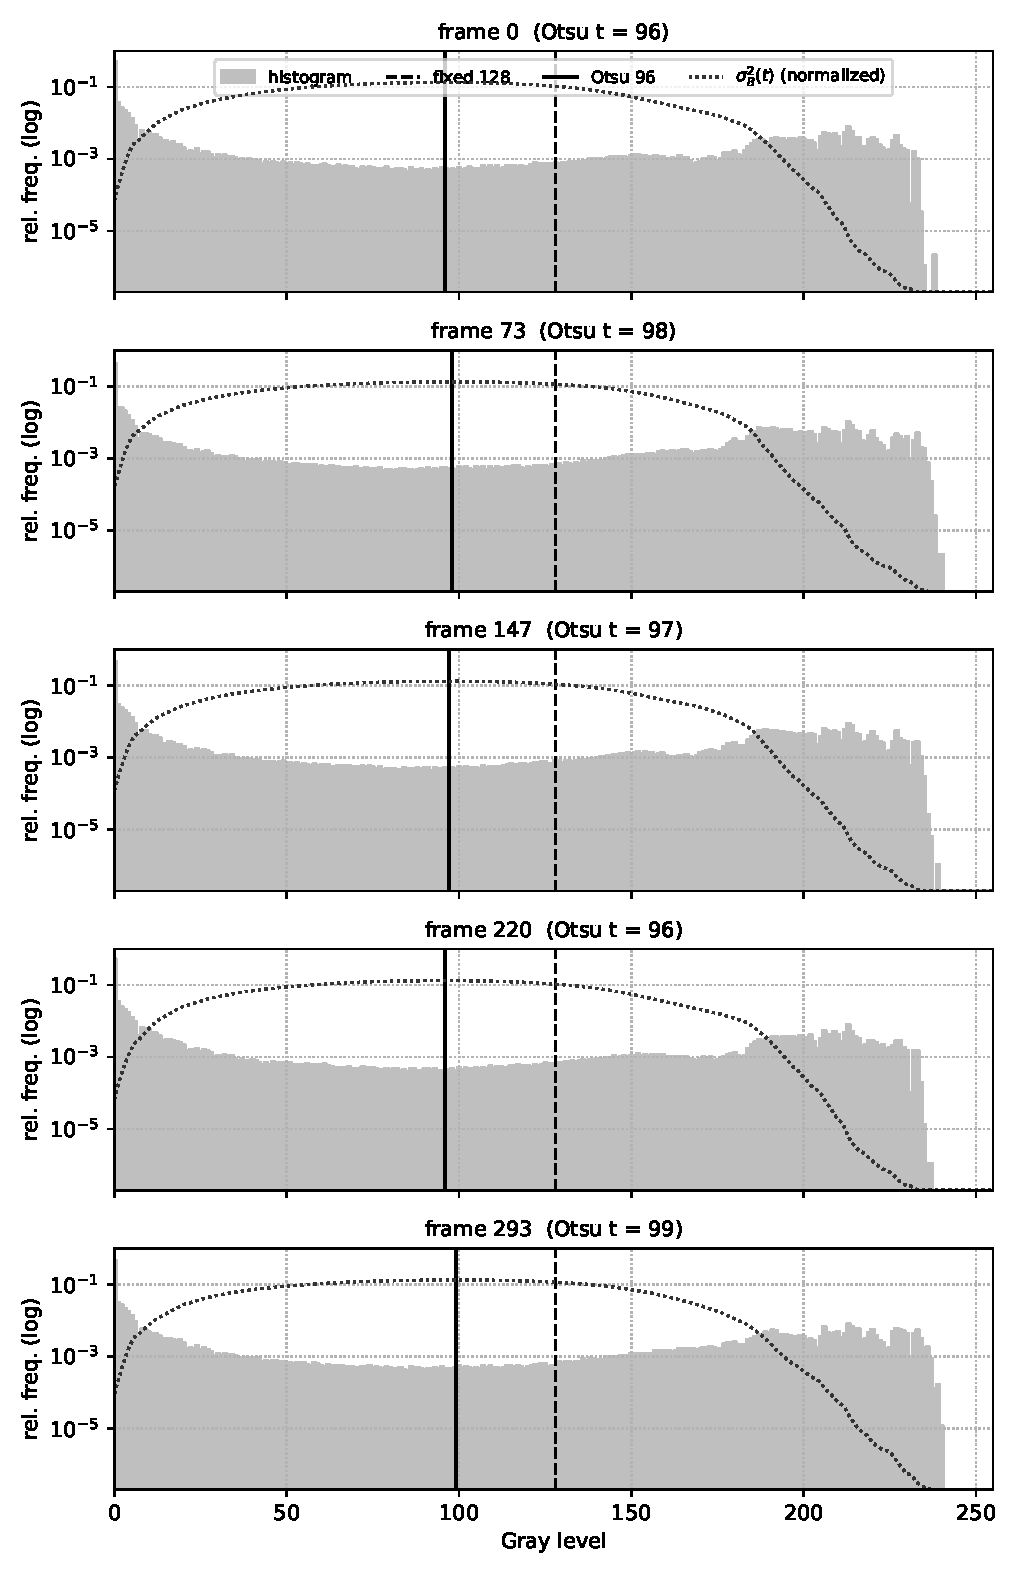
\includegraphics[width=0.82\linewidth]{../experiments/figures/exp06_hist_thresholds.pdf}
\caption{5 フレームのグレースケールヒストグラム(縦軸対数)と閾値の位置。
破線は固定閾値 128、実線は Otsu 閾値、点線はクラス間分散
$\sigma_B^2(t)$(式 \ref{eq:b6-sigmab}、最大値で正規化)である。}
\label{fig:b6-hist}
\end{figure}

図 \ref{fig:b6-hist} から、Cat 動画のヒストグラムは 0 付近(黒い毛)と
190〜250 付近(白い毛と明るい背景)に山を持つ双峰型で、その間に相対度数
$10^{-3}$ 程度の広く浅い谷が続くことが分かる。Otsu 閾値は 5 フレームとも
95〜100 で谷の左寄りに位置し、固定閾値 128 も同じ谷の中にある。
$\sigma_B^2(t)$ の曲線は谷のほぼ全域で平坦に近く、最大点付近の勾配が
小さい。これは、ヒストグラムのわずかな変動で式 \ref{eq:b6-argmax} の
最大位置が動きやすい構造であることを意味し、後述する閾値のフレーム間
ゆらぎの原因になる。

\begin{figure}[htbp]
\centering
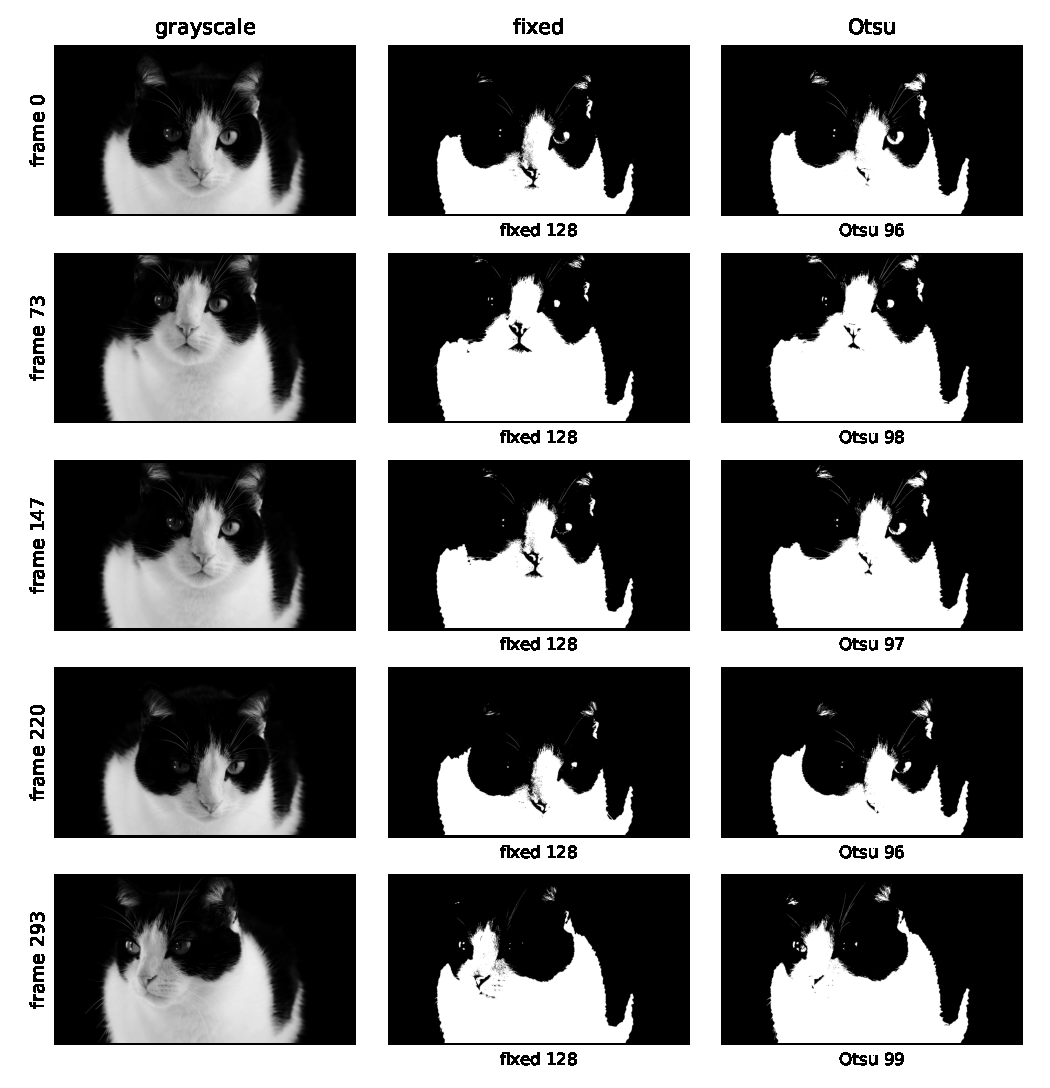
\includegraphics[width=0.92\linewidth]{../experiments/figures/exp06_binarize_compare.pdf}
\caption{固定閾値 128 と Otsu 閾値による二値化結果の比較。左列は
グレースケール、中列は固定 128、右列はフレーム毎 Otsu である。}
\label{fig:b6-binarize}
\end{figure}

図 \ref{fig:b6-binarize} に両方式の二値化結果を並置する。両閾値が
同じ谷に入っているため大局的な白黒パターンはほぼ共通であり、差は
谷内の中間調(96〜127)の画素に限られる。Otsu の方が閾値が低いぶん、
暗部の毛の細部がやや多く白側に出ており、白画素率の差は 5 フレームの
いずれでも 1.5〜1.9 ポイント(表 \ref{tab:b6-samples})、全フレーム
平均では 1.7 ポイント(28.50 \% 対 26.78 \%)である。固定 128 が
本動画で視覚的に破綻しないのは、入力のヒストグラムが幅広く浅い谷を
持つ双峰型であり、谷の中であれば閾値がどこにあっても結果が大きく
変わらないためである。

\subsubsection{Otsu 閾値の時間変化}

図 \ref{fig:b6-series} に全 294 フレームの Otsu 閾値の推移を示す。
統計量は、平均 97.15、標準偏差 1.34、最小 95、最大 100(範囲 5)で
あった。また、全フレームのヒストグラムを合算して求めた動画一括
Otsu 閾値は 97 で、フレーム毎閾値の平均 97.15 とほぼ一致した。

\begin{figure}[htbp]
\centering
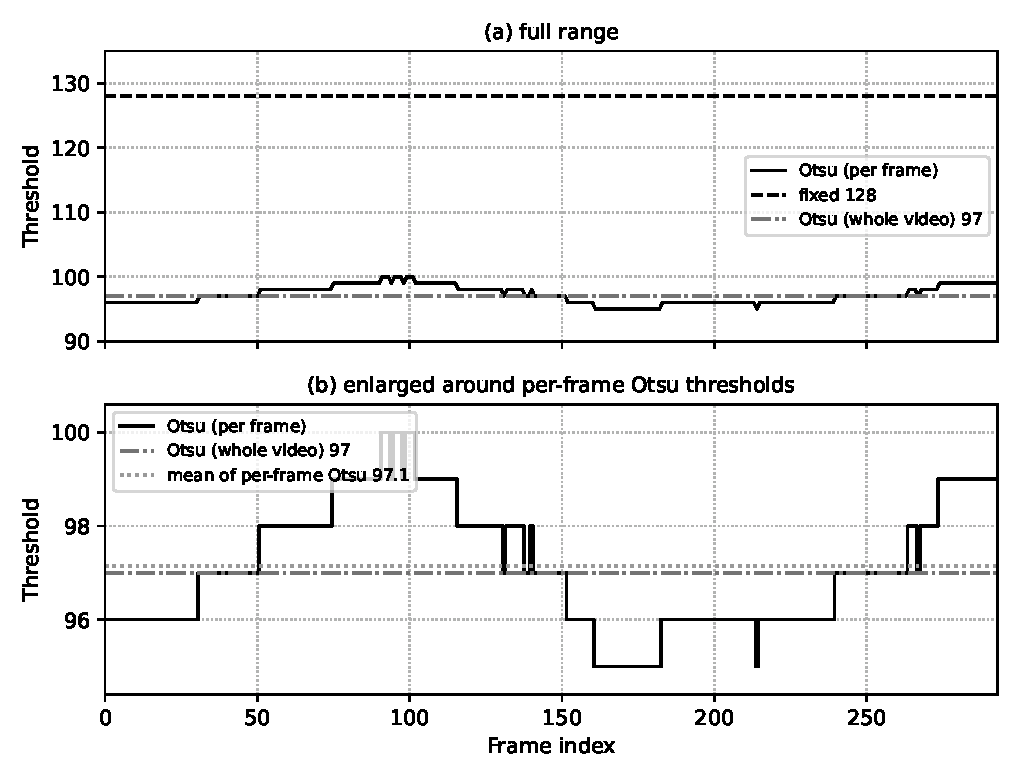
\includegraphics[width=0.85\linewidth]{../experiments/figures/exp06_threshold_series.pdf}
\caption{Otsu 閾値の推移。(a) は固定 128(破線)・動画一括 Otsu
(一点鎖線)との比較、(b) はフレーム毎 Otsu 閾値付近の拡大である。}
\label{fig:b6-series}
\end{figure}

図 \ref{fig:b6-series}(a) のとおり、固定閾値 128 は全フレームで
Otsu 閾値より 28 以上大きく、判別分析の基準(式 \ref{eq:b6-argmax})から
見れば一貫して最適点から外れている。一方、図 \ref{fig:b6-series}(b) の
拡大から、フレーム毎 Otsu の閾値は 95〜100 の間を階段状に移動し、
隣接フレーム間の変化 $|\Delta t|$ は平均 0.085、最大でも 1 レベルに
とどまることが分かる。本動画は場面転換のない単一ショットで照明も
安定しているため閾値の変動は小さいが、変化が「1 レベルの離散的な
跳び」として起こる点が固定閾値との本質的な違いであり、次項で述べる
ちらつきの発生源になる。

\subsubsection{時間方向の安定性 --- ちらつきの定量化}

二値化動画の見えの安定性を評価する代理指標として、各フレームの
白画素率 $r_k$(フレーム $k$ の白画素数を総画素数で割った値)を
3 方式で計算し、(1) 全フレームにわたる分散(動画全体での変動の
大きさ)と、(2) 隣接フレーム間変化量 $|\Delta r| = |r_{k+1} - r_k|$ の
平均(フレーム間の跳び、すなわちちらつきの大きさ)を比較した。
結果を表 \ref{tab:b6-stability} と図 \ref{fig:b6-ratio} に示す。

\begin{table}[htbp]
\centering
\caption{白画素率の時間方向の統計(294 フレーム。分散・標準偏差は
ddof$=0$、$|\Delta r|$ はポイント)}
\label{tab:b6-stability}
\begin{tabular}{lrrrrr}
\hline
方式 & 平均 [\%] & 分散 & 標準偏差 [pt] & 平均 $|\Delta r|$ [pt] &
最大 $|\Delta r|$ [pt] \\
\hline
固定 128(課題 8) & 26.78 & $1.527 \times 10^{-3}$ & 3.91 & 0.168 & 1.00 \\
フレーム毎 Otsu & 28.50 & $1.505 \times 10^{-3}$ & 3.88 & 0.175 & 1.08 \\
動画一括 Otsu(97) & 28.51 & $1.544 \times 10^{-3}$ & 3.93 & 0.175 & 1.07 \\
\hline
\end{tabular}
\end{table}

\begin{figure}[htbp]
\centering
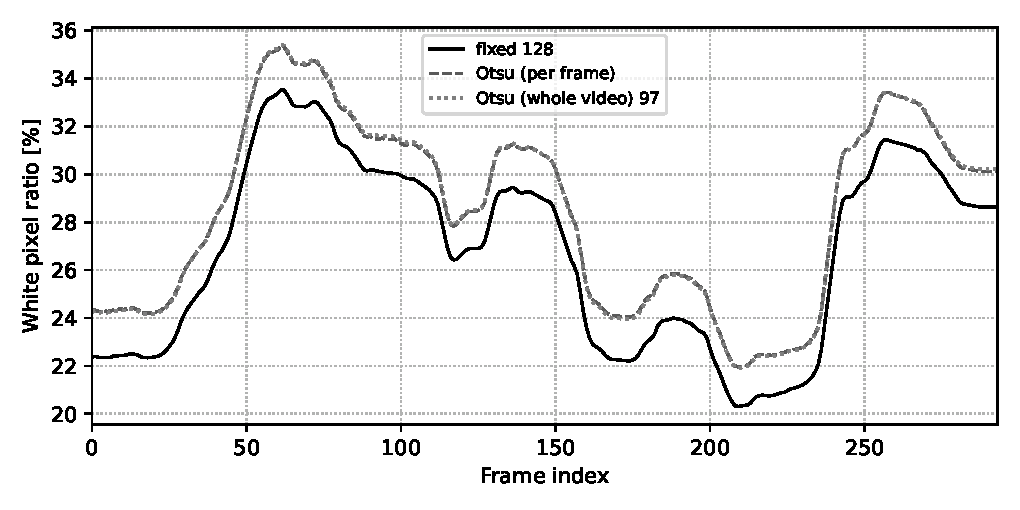
\includegraphics[width=0.85\linewidth]{../experiments/figures/exp06_white_ratio.pdf}
\caption{白画素率の推移。実線は固定 128、破線はフレーム毎 Otsu、
点線は動画一括 Otsu(閾値 97)である。}
\label{fig:b6-ratio}
\end{figure}

表 \ref{tab:b6-stability} から次の 3 点が読み取れる。第一に、
白画素率の分散は 3 方式でほぼ等しく(フレーム毎 Otsu は固定 128 の
0.986 倍、動画一括 Otsu は 1.011 倍)、図 \ref{fig:b6-ratio} の 3 本の
曲線もほぼ平行に上下する。すなわち白画素率の変動は被写体の動きによる
画面内容の変化が支配的であり、閾値方式の選択は動画全体での変動幅を
ほとんど変えない。むしろ同じ動作点(閾値 97 近傍)で比べると、
フレーム毎 Otsu の分散($1.505 \times 10^{-3}$)は閾値を固定した
動画一括 Otsu($1.544 \times 10^{-3}$)より 2.5 \% 小さい。これは
明るさが変わったフレームで閾値が同方向に追従し、白画素率の変化を
打ち消す負帰還として働くためであり、フレーム毎 Otsu の適応性が
長時間スケールの安定性をわずかに改善することを示す。

第二に、ちらつきの指標である平均 $|\Delta r|$ は、フレーム毎 Otsu が
0.175 ポイントで固定 128(0.168 ポイント)の 1.040 倍であった。ただし
閾値が時間不変の動画一括 Otsu も 1.041 倍であることから、この増分の
大半はフレーム毎の適応ではなく動作点の違い(閾値 97 付近は 128 付近
より内容変化に対する白画素率の感度がわずかに高い)に由来する。

第三に、閾値の切り替わりがちらつきに与える影響を切り分けるため、
293 の隣接フレーム遷移を「Otsu 閾値が変化した遷移($|\Delta t| = 1$、
25 回)」と「変化しなかった遷移(268 回)」に分けて $|\Delta r|$ を
比較した(表 \ref{tab:b6-flicker})。

\begin{table}[htbp]
\centering
\caption{閾値変化の有無による隣接フレーム間白画素率変化 $|\Delta r|$ の比較}
\label{tab:b6-flicker}
\begin{tabular}{lrrrr}
\hline
条件 & 遷移数 & 平均 $|\Delta r|$ Otsu [pt] & 平均 $|\Delta r|$ 固定 128 [pt] & 比 \\
\hline
閾値変化あり($|\Delta t| = 1$) & 25 & 0.2115 & 0.1987 & 1.065 \\
閾値変化なし($\Delta t = 0$) & 268 & 0.1713 & 0.1652 & 1.037 \\
\hline
\end{tabular}
\end{table}

表 \ref{tab:b6-flicker} のとおり、固定 128 に対する超過は、閾値が
変化しなかった遷移で 1.037 倍、変化した遷移では 1.065 倍と拡大する。
すなわちフレーム毎 Otsu の閾値切り替えは、同じ内容変化に対して
白画素率の跳びを確かに増やしており、これが「フレーム毎の自動閾値は
ちらつきを生む」というトレードオフの実測値である。一方でその絶対量が
小さい(超過 0.013 ポイント程度)のは、本動画では (1) 閾値の変化が
293 遷移中 25 回、かつ 1 レベルに限られること、(2) 閾値が動く谷の
相対度数が $10^{-3}$ 程度と低く、閾値 1 レベル分で反転する画素が
全体の約 0.1 \% にとどまること(図 \ref{fig:b6-hist})、(3) 閾値の
上昇は画面が明るくなったフレームで起こりやすく、内容変化による
白画素率の増加を部分的に打ち消す方向に働くこと、による。逆に言えば、
場面転換や照明変動を含む動画、あるいは谷の密度が高い(または谷が
明確でない)ヒストグラムを持つ動画では、閾値の跳び幅と 1 レベルあたりの
反転画素数の両方が大きくなり、ちらつきは本実験よりはるかに顕著に
なると考えられる。大津の方法が双峰的で対称な分布を暗黙に仮定しており、
分布形状によっては最適点が不安定になることは、クラス間分散の改良を
提案した 2022 年の研究 \cite{b6-lognormal} でも指摘されている。

\subsubsection{設計選択の評価と改善案}

以上の結果から、課題 8 の固定閾値 128 とその代替案は次のように
評価できる。固定 128 は、本動画に限れば閾値がヒストグラムの谷に
収まるため視覚的に破綻せず、ちらつきも最小である。しかしこれは
入力が「幅広く浅い谷を持つ双峰型ヒストグラム」であることに依存した
結果であり、判別分析の基準では全フレームで最適点(95〜100)から
28 以上外れている。露出の異なる動画(たとえば全体に暗い映像)では
谷の位置が 128 から離れ、大半の画素が一方のクラスに潰れる。大局的
閾値法一般が照明の不均一や分布の重なりに弱いことはレビュー
\cite{b6-binreview} でも整理されており、入力非依存の固定値はその
最も脆弱な形態である。

フレーム毎 Otsu は入力への適応性を獲得する代わりに、閾値切り替え時の
ちらつき(表 \ref{tab:b6-flicker} の超過 1.065 倍)を導入する。
本実験の動画一括 Otsu は両者の中間に位置する実用的な折衷案であり、
(1) 閾値 97 がフレーム毎閾値の平均 97.15 とほぼ一致して適応性を保ち、
(2) 閾値が時間不変であるため閾値起因のちらつきが原理的に生じない。
実装上も、合算ヒストグラムから求めた閾値を {\tt binarize\_frame} の
引数 {\tt threshold} に渡すだけでよく、課題 8 で採用した「フレーム
変換関数と動画入出力の分離」という高階関数設計をそのまま活かせる。
必要な追加コストは、二値化に先立って全フレームのヒストグラムを
集計する 1 パス(または閾値決定を先頭の数フレームで代用する近似)で
ある。したがって、単一ショットの動画を対象とする限り、動画一括
Otsu を既定とし、場面転換のある動画ではショット単位(課題 7 の
変わり目検出で区切った区間単位)に閾値を決め直す設計が、固定 128 と
フレーム毎 Otsu の双方の欠点を避ける改善案として妥当であると
結論できる。
